\documentclass[final]{fhnwreport}       %[mode] = draft or final
                                        %{class} = fhnwreport, article, 
                                        %          report, book, beamer, standalone
%%---Main Packages-----------------------------------------------------------------------
\usepackage[english, ngerman]{babel}	%Mul­tilin­gual sup­port for LaTeX
\usepackage[T1]{fontenc}				%Stan­dard pack­age for se­lect­ing font en­cod­ings
\usepackage[utf8]{inputenc}				%Ac­cept dif­fer­ent in­put en­cod­ings
\usepackage{lmodern}                    %The newer Font-Set
\usepackage{textcomp}					%LaTeX sup­port for the Text Com­pan­ion fonts
\usepackage{graphicx} 					%En­hanced sup­port for graph­ics
\usepackage{float}						%Im­proved in­ter­face for float­ing ob­jects
\usepackage{ifdraft}                    %Let you check if the doc is in draft mode

%%---Useful Packages---------------------------------------------------------------------
\usepackage[pdftex,dvipsnames]{xcolor}  %Driver-in­de­pen­dent color ex­ten­sions for LaTeX
\usepackage{csquotes}                   %Simpler quoting with \enquote{}
\usepackage{siunitx} 					%A com­pre­hen­sive (SI) units pack­age
\usepackage{listings}					%Type­set source code list­ings us­ing LaTeX
\usepackage[bottom]{footmisc}			%A range of foot­note op­tions
\usepackage{footnote}					%Im­prove on LaTeX's foot­note han­dling
\usepackage{verbatim}					%Reim­ple­men­ta­tion of and ex­ten­sions to LaTeX ver­ba­tim
%\usepackage[textsize=footnotesize,disable]{todonotes} %Mark­ing things to do in a LaTeX doc­u­ment
\usepackage[colorinlistoftodos,prependcaption,textsize=tiny]{todonotes} %Mark­ing things to do in a LaTeX doc­u­ment
\usepackage{titling}					%Control over the typesetting of the \maketitle command
\usepackage{pbox}

%%---Tikz Packages-----------------------------------------------------------------------
\usepackage{standalone}
\usepackage{tikz}
\usepackage{circuitikz}
\usetikzlibrary{arrows}
\usetikzlibrary{calc}
\usetikzlibrary{intersections}

%%---Math Packages-----------------------------------------------------------------------
\usepackage{amsmath}					%AMS math­e­mat­i­cal fa­cil­i­ties for LaTeX
\usepackage{amssymb}					%Type­set­ting symbols (AMS style)
%\usepackage{array}						%Ex­tend­ing the ar­ray and tab­u­lar en­vi­ron­ments
%\usepackage{amsthm}					%Type­set­ting the­o­rems (AMS style)

%%---Table Packages----------------------------------------------------------------------
\usepackage{tabularx}					%Tab­u­lars with ad­justable-width columns
\usepackage{longtable}
\usepackage{multirow}					%Create tab­u­lar cells span­ning mul­ti­ple rows
\usepackage{multicol}					%In­ter­mix sin­gle and mul­ti­ple columns

%%---PDF / Figure Packages---------------------------------------------------------------
\usepackage{pdfpages}					%In­clude PDF doc­u­ments in LaTeX
\usepackage{pdflscape}					%Make land­scape pages dis­play as land­scape
\usepackage{subfig}					    %Fig­ures di­vided into sub­fig­ures

%%---Other Packages----------------------------------------------------------------------
%\usepackage{xargs}                     %De­fine com­mands with many op­tional ar­gu­ments


%%---Bibliography------------------------------------------------------------------------
\usepackage[style=ieee,urldate=comp,backend=biber]{biblatex}
\addbibresource{literature/bibliography.bib}

%%---Main Settings-----------------------------------------------------------------------
\graphicspath{{./graphics/}}			%Defines the graphicspath
\geometry{twoside=false}				    %twoside=false disables the "bookstyle"
\setlength{\marginparwidth}{2cm}
\overfullrule=5em						%Creates a black rule if text goes over the margins => debugging




%%---User Definitions--------------------------------------------------------------------
%%Tabel-Definitions: (requires \usepackage{tabularx})
\newcolumntype{L}[1]{>{\raggedright\arraybackslash}p{#1}}    %column-width and alignment
\newcolumntype{C}[1]{>{\centering\arraybackslash}p{#1}}
\newcolumntype{R}[1]{>{\raggedleft\arraybackslash}p{#1}}

%%---Optional Package Settings-----------------------------------------------------------
%Listings-Settings: (requires \usepackage{listings}) => Example with Matlab Code
\lstset{language=Matlab,%
    basicstyle=\footnotesize\ttfamily,
    breaklines=false,%
    morekeywords={switch, case, otherwise},
    keywordstyle=\color{Blue},%
    tabsize=2,
    %morekeywords=[2]{1}, keywordstyle=[2]{\color{black}},
    identifierstyle=\color{Black},%
    stringstyle=\color{Purple},
    commentstyle=\color{Green},%
    showstringspaces=false,%without this there will be a symbol in the places where there is a space
    numbers=left,%
    numberstyle={\tiny \color{black}},% size of the numbers
    numbersep=9pt, % this defines how far the numbers are from the text
    %emph=[1]{word1, word2,...},emphstyle=[1]\color{red}
}							

% Hurenkinder und Schusterjungen verhindern ( kein scherz Google es)
\clubpenalty10000
\widowpenalty10000
\displaywidowpenalty=10000				                %loads all packages, definitions and settings											
\title{\textbf{Entwicklung einer Entry-Level Audioeffektbox mit einem ARM Cortex-M4F DSP}}  		        %Project Title
\author{Burkhardt Simon, Studer Mischa} %Document Type => Technical Report, ...
\date{\today}          				   %Place and Date

\begin{document}

%%---TITLEPAGE---------------------------------------------------------------------------------
\thispagestyle{empty}
%	\ohead{\includegraphics[scale=0.5]{Bilder/Logo_FHNW.jpg}}
	\begin{figure}
		 \vspace*{-\topskip}\vspace*{-\headsep}
		
\includegraphics[scale=1]{fhnw_ht_logo_de.pdf}
	\end{figure}
	\begin{center}
		\vspace*{2cm}
		{\huge{\textbf{\thetitle}}}\\
		\vspace*{0.5cm}
		
		{\scshape\Large Fachbericht: Projekt 5 - \theauthor \\} \Large{\today}
		\vfill
		\begin{normalsize}
			{\begin{tabbing}
					\textbf{Betreuung:} \hspace{5cm}\= Prof. Dr. Markus Hufschmid\\
					
					%\\[0.8cm]
					%\textbf{Auftraggeber:} 
					%\>Prof. Dr. Markus Hufschmid\\
					
					\\[0.8cm]
					\textbf{Team:} \> Simon Burkhardt\\ 
					\> Mischa Studer\\
					\\[0.8cm]
					\\[0.8cm]
					\textbf{Studiengang:} \>Elektro- und Informationstechnik
					\\[0.8cm]	\textbf{Semester:} \>Herbstsemester 2019
			\end{tabbing}}
		\end{normalsize}
		\vfill
	\end{center}
\clearpage

%%---ABSTRACT----------------------------------------------------------------------------
\selectlanguage{ngerman}				%ngerman or english
\thispagestyle{empty}
\begin{otherlanguage}{english}
\include{sections/abstract}
\end{otherlanguage}

%%---TABLE OF CONTENTS-------------------------------------------------------------------
\pagenumbering{Roman}		
\selectlanguage{ngerman}				%ngerman or english
\tableofcontents
\clearpage

%%---TEXT--------------------------------------------------------------------------------

\pagenumbering{arabic}
\section{Einleitung}
\label{sec:Einleitung}

Ein Amateurfunker hat während des Funkbetriebs immer wieder mit verschiedenen Störgeräuschen zu kämpfen die die Verständlichkeit der Verbindung erheblich beeinflussen. Genauso ist es für einen Hobbymusiker mühsam 19-Zoll Racks mit analogen Effekt-Geräten von Gig zu Gig zu schleppen, wenn er seine Musik nur mit ein paar simplen Audioeffekten versetzen möchte. In beiden Bereichen fehlt auch meistens das Budget und der Platz für teures analoges Equipment.\\
Hier bietet sich ein perfektes Anwendungsgebiet für digitale Signalverarbeitung. Jedoch sind auch handelsübliche digitale Effektgeräte meist nur für sehr spezifische Anwendungen konzipiert und kommen selten wirklich handlich daher.

Deswegen ist es das Ziel in diesem Projekt eine handliche DSP Einheit zu entwerfen, die mit einem schnellen modernen Microcontroller geeignete Effekte rechnen kann. Im Gegensatz zum Vorgängerprojekt, das mit einem dsPIC33 ausgestattet war und bis anhin im MicroCom Labor eingesetzt wurde, wird das neue Board mit einem ARM Cortex M4 Prozessor bestückt welcher dank seiner Floating-Point-Unit eine schnellere Verarbeitung von Signalen ermöglicht. Für die AD/DA-Wandlung sorgt ein TLV320 Codec um die Audio-Signale zuverlässig hin und her zu wandeln.

Die Vorteile einer Lösung  mittels Microcontroller sind so zahlreich wie offensichtlich. Dank der Vielseitigkeit der digitalen Signalverarbeitung können je nach Bedarf beliebige Effekte programmiert und auf das Board geflasht werden \footnote{In diesem Projekt ist es das Ziel die Hardware zu entwerfen und die Software soweit vorzubereiten, dass ein einfaches Audio-In/Audio-Out möglich ist. In einem späteren Projekt erst soll ein Tool entwickelt werden, welches die entsprechenden Effekte berechnet und aufs Board lädt.}. Der Prozessor inkl. Codec plus der Audio- und Kommunikations-Schnittstellen brauchen weder viel Platz, noch sind sie teuer. Die derzeitige Lösung ist auf einem 7x10cm PCB mit einem Budget-Rahmen von 50SFr realisiert worden. Ein DSP-Board mittels Microcontroller ist also die perfekte Lösung für Hobby-Anwendungen im Bereich Funk oder Musik.

Da die Bedienelemente mit je zwei Tasten, zwei Rotary Encoders und zwei 1.96inch Displays eher minimalistisch gehalten sind, können mehere DSP-Boards beliebig kaskadiert werden. Wie bei einem Puzzleteil werden die Boards ineinandergesteckt und über einen analogen Audio-Stecker wird das Signal von Board zu Board weitergeschlauft und weiterverarbeitet. So bleibt das System modular und kann für beliebige Anwendungen eingesetzt werden.

Das erarbeitete DSP-Board funktioniert erwartungsgemäss. Es ist möglich ein Audio-Signal einzuspeisen welches nach erfolgreicher AD/DA-Wandlung wieder am Audio-Ausgang anliegt. Die verschiedenen Ein-/Ausgänge sowie deren Pegel sind anwählbar über ein einfaches Menu. Zusätzlich wurde sogar ein FIR-Filter mit verstellbarer Grenzfrequenz implementiert.

%Kleine Fehler in der Analog-Schaltung haben sich eingeschlichen welche Verbesserungspotential bieten, jedoch keinen entscheidenden Einfluss auf die Funktion haben.

Die folgende Facharbeit ist in Analyse/Konzept, Hardware, Software, Validierung und Status/Verbesserungen unterteilt. Erst wird das angedachte Konzept grob erklärt und dessen Funktionsweise erläutert wonach detailliert auf die Umsetzung in den Teil-Bereichen Hardware und Software eingegangen wird. In den letzten beiden Kapiteln werden Teils-Systeme mit entsprechenden Messungen auf ihre Genauigkeit und Funktionalität untersucht und zum Schluss der momentane Status und mögliche Verbesserungen für weiterführende Projekte dargelegt.

%Das derzeit verwendete DSP Board für den Unterricht im MicroCom Labor basiert auf einem dsPIC33 mit Fixed-Point-Recheneinheit. Die neuen ARM Prozessoren bieten ab der Cortex-M4 Serie eine Floating-Point-Unit (FPU) und ermöglichen dadurch eine schnellere Verarbeitung von Signalen. \\
%
%Aus diesem Grund wird die Hardware des DSP Boards überarbeitet und soll mit einem ARM Cortex-M4 Microcontroller ausgestattet werden. Der Schaltungsaufwand beschränkt sich auf die wesentlichen Funktionen. Diese beinhalten die MCU, einen Codec für die AD/DA Wandlung, die Audio-Steckverbinder und die Bedienelemente des HMI. \\
%
%Im Bereich Amateurfunk und Hobbymusik besteht oft ein Bedürfnis nach einer einfachen Möglichkeit, ein Audiosignal mit einem Effekt zu verändern.
%So kann es sein, dass ein Amateurfunker mit einem Notch-Filter einen Störton unterdrücken möchte. Als Musiker möchte man mit einer Effektbox einen Reverbeffekt erzeugen.
%Effektgeräte und Filter am Markt sind oft zu einem Premiumpreis erhältlich.
%Dieses Projekt hat zum Ziel, eine günstige Alternative zu diesen Geräten zu bieten.
%
%
%Heute bieten die DSP Funktionen in der ARM Cortex-M4 Architektur einegünstige Möglichkeit Signalverarbeitung auf Microcontrollerebene zu betreiben. 
%Der Rahmen dieses Projektes umfasst die Entwicklung der Hard- und Firmware eines DSP Boards mit ARM Cortex-M4 Microcontroller. 
%Das Gerät wird mit Bedienelementen wie 2 Dreh


\clearpage
\section{Analyse und Konzept}
\label{sec:Analyse_Kozept}

Die mit dem betreuenden Fachdozenten Prof. Dr. Markus Hufschmid erarbeiteten Projektziele sind im Pflichtenheft hinterlegt (einzusehen im Appendix \ref{app:Pflichtenheft}).  Nachfolgend ist das erarbeitete Lösungskonzept näher erklärt welches zur Erreichung selbiger führen sollte.

\subsection{Produktbeschreibung}
\label{sec:Produktbeschreibung}







\section{Ziele}
\label{sec:Ziele}

\subsection{Harte Ziele}

\begin{table}[H]
\begin{tabular}{|l|l|l|ll}
\cline{1-3}

\textbf{Nr} & \textbf{Ziel} & \textbf{Erreichungsgrad} &  &  \\ \cline{1-3}
1.1         & Microcontroller mit Coretx-M4F Architecktur & erfüllt/nicht erfüllt    &  &  \\ \cline{1-3}
1.2         & Audio Passthrough von Line-In nach Line-Out                                                     & erfüllt/nicht erfüllt    &  &  \\ \cline{1-3}
1.3         & \begin{tabular}[c]{@{}l@{}}Audio Schnittstelle (analog) \\ - Line-IN \\ - Line OUT\end{tabular} & erfüllt/nicht erfüllt    &  &  \\ \cline{1-3}
1.4         & 2 Stk. Drehencoder für HMI                                                                      & erfüllt/nicht erfüllt    &  &  \\ \cline{1-3}
1.5         & 2 Stk. Taster für HMI                                                                           & erfüllt/nicht erfüllt    &  &  \\ \cline{1-3}
1.6         & 1 Display zur Anzeige des Funktionsmodus                                                        & erfüllt/nicht erfüllt    &  &  \\ \cline{1-3}
1.7         & Microcontroller ohne Debugger über USB programmierbar                                           & erfüllt/nicht erfüllt    &  &  \\ \cline{1-3}
\end{tabular}
\end{table}

\subsection{Weiche Ziele}

\begin{table}[H]
\begin{tabular}{|l|l|l|ll}
\cline{1-3}
\textbf{Nr} & \textbf{Ziel}                                                                                   & \textbf{Erreichungsgrad} &  &  \\ \cline{1-3}
2.1         & Anzahl Layer der Leiterplatte                                                     & ${n_{Layer} \leq 2}$    &  &  \\ \cline{1-3}
2.2         & \begin{tabular}[c]{@{}l@{}}Bauteile sind Handbestückbar \\ - SMD passiv $\geq$ 0603 \\ - SMD cases: keine QFN / BGA\end{tabular} & erfüllt/nicht erfüllt &  &  \\ \cline{1-3}
2.3         & Stromverbrauch erlaubt Betrieb über USB 2.0 Speisung & ${I_{USB} \leq 0.5A}$    &  &  \\ \cline{1-3}
2.4         & \begin{tabular}[c]{@{}l@{}}Audio Schnittstelle (analog) \\ - Headphone OUT \\ - Microphone IN\end{tabular} & erfüllt/nicht erfüllt    &  &  \\ \cline{1-3}
2.5         & \begin{tabular}[c]{@{}l@{}} Audio Verbindung (digital) \\ - IN / OUT Board-to-Board Kommunikation \\ Kaskadierung mehrerer Boards\end{tabular} & erfüllt/nicht erfüllt    &  &  \\ \cline{1-3}
2.6         & Akkubetrieb möglich & erfüllt/nicht erfüllt    &  &  \\ \cline{1-3}
2.7         & zusätzliche (farbige) LEDs als Anzeige des Betriebsmodus & erfüllt/nicht erfüllt    &  &  \\ \cline{1-3}
2.8         & Materialkosten inkl. PCB pro Stück bei 10 Stk. & ${k \leq 50 CHF}$    &  & \\ \cline{1-3}
\end{tabular}
\end{table}

\subsection{Nicht Ziele}

\begin{table}[H]
\begin{tabular}{|l|l|l|ll}
\cline{1-3}
\textbf{Nr} & \textbf{Ziel}                     & \textbf{Erreichungsgrad} &  &  \\ \cline{1-3}
3.1         & DSP Board für den Unterricht      & erfüllt/nicht erfüllt    &  &  \\ \cline{1-3}
3.2         & Aufwändiges Gehäuse               & erfüllt/nicht erfüllt    &  &  \\ \cline{1-3}
\end{tabular}
\end{table}


\subsection{Lösungskonzept}
\label{sec:Loesungskonzept}

In diesem Abschnitt werden die Anforderungen and die einzelnen Teilaspekte aufgelistet und die Spezifikationen mehrerer Varianten verglichen.



\subsubsection{Anforderungen an Microcontroller}
\label{sec:Konzept_Microcontroller}

Die an den Prozessor gestellten Anforderungen sind ein ARM-Cortex M4 Core mit DSP und FPU sowie Schnittstelle(n) zur Kommunikation mit dem Audio Codec. 
Dabei wird aufgrund der genaueren Samplingrate der Codec als Master betrieben und der DSP als Slave.
Der DSP muss also keine genaue Clock zur Verfügung stellen. 
Auf eine Cortex-M7 Architektur wird verzichtet, weil ab diesem Punkt auch ein Single-Board Computer (vgl. Raspberry Pi) eingesetzt werden kann.
Eine Tacktfrequenz von 200MHz ist wünschenswert, jedoch befinden sich die Cortex-M4 Prozessoren mit 200MHz auf dem selben Preisniveau von Cortex-M7 Microcontrollern.



\subsubsection{Konzept USB Akkuladeregler IC}
\label{sec:Konzept_Charger}

Ein weiches Ziel ist die Autonomie ohne externe Energieversorgung. 
Dazu soll ein Akkumulator genügend Energie liefern, um die Schaltung während einiger weniger Stunden (live-Konzert) zu betreiben. 
Der Ladestrom soll nicht grösser als die über USB-2.0 zugelassenen $2.0\si{A}$ betragen.





\subsection{Kaskadierung mehrerer Boards}
\label{subsec:Konzept_Kaskadierung}

Mehrere DSP-Boards sollen untereinander kaskadierbar sein, um das bearbeite Audio-Signal auf einem nächsten Board weiter zu verarbeiten. Auf eine digitale Schnittstelle wird in Absprache mit dem Auftraggeber, wegen der aufwändigen Clock-Synchronisation verzichtet. Das Signal wird analog weitergereicht, was in mehr analogem Rauschen resultiert. Dieser Effekt wird durch die kurzen Leitungen von Board zu Board minimal gehalten. Da die Gefahr besteht, dass der Benutzer jeweilige Link-Kabel verlegt oder zumindest nicht in nützlicher Frist zur Hand hat, wird die Kaskadierung mit einer Steckverbindung gelöst. Dabei werden zwei Boards direkt nebeneinander (Kante an Kante) zusammengesteckt.


\begin{table}[H]
	\centering
	\begin{tabular}{|c|c|c|c|}
		\hline
		\textbf{Specification} & \textbf{Mill-Max 868}             & \textbf{Pin Header 2x3} & \textbf{AVX 9159} \\ \hline
		Preis         & 5.26 + 7.00 (F/M 3P.)& 1.50 + 0.80 (M/F 6P.)&1.05 + 0.78 (F/M 3P)         \\ \hline
	\end{tabular}
	\caption{Preisvergleich der analogen Steckverbinder}
	\label{tab:stecker}
\end{table}

Da die verschiedenen Steckverbinder in \ref{tab:stecker} in Anzahl Leitungen alle das gleiche bieten, ist hier vor allem der Preis entscheidend. Der \textbf{AVX 9159}, welcher ursprünglich für LED-Schienen eingesetzt wird, ist mit Abstand der günstigste und eignet sich ebenso für eine Audio-Anwendung.



%Das Audio Signal wird von einem Board zum nächsten jeweils analog weitergereicht. 
%Der Steckverbinder soll kleiner als D-Sub sein. 
%Auf eine digitale Schnittstelle wird in Absprache mit dem Auftraggeber,  wegen der aufwändigen Clock-synchronisation und der Kosten für Steckverbinder (vgl. Optisch Toslink) verzichtet. 
%
%\todo{SB: Kaskadierungskonzept
%Weitergabe von analogem Signal und dadurch entstehendes mehrmaliges Wandeln ist unsauber aber analog ist einfach..oder so AVX-Stecker/Audio-Switch}

\clearpage

\clearpage
%\section{Schluss}
\label{sec:Schluss}
\todo[inline]{Gegenlesen - Fertig - MR -  In diesem Kapitel steht die Zusammenfassung des Resultats und inwiefern die Projektziele damit erfüllt sind (mit Verweis auf die Validierung). Ebenfalls wird das Weiterentwicklungspotential aufgezeigt. - A: MR}

Anhand der Mechanik des 3D Druckers Ender 3 Pro und der eigens gefertigten Steuerung konnte ein robuster, leistungsfähiger und einfach zu bedienender Drucker entwickelt und in Betrieb genommen werden (siehe Kapitel \ref{sec:Validierung}). Neben allen definierten Sollzielen konnten auch alle Wunschziele umgesetzt werden.

Der Benutzer kann seine G-Code Files nun nicht nur per SD-Karte, sondern auch per Fernzugriff über das Webinterface auf den Drucker laden und den Druck auch gleich starten. Über den Druckfortschritt wird er auf dem Display des Druckers oder auch auf dem Webinterface informiert. Die beiden horizontalen Achsen des Druckers (X- und Y-Achse) werden ohne Endschalter referenziert. Dadurch ist die Anzahl der  Sensoren reduziert.
Der verwendete 32-Bit Prozessor verfügt über genug Rechenleistung, sodass zukünftig auch Erweiterungen vorgenommen werden können, die rechenaufwändig sind. Des Weiteren können Updates der Firmware über das Webinterface getätigt werden. Ungenutze Pins des Prozessors sind auf Headers geführt, wodurch die Implementierung eines weiteren Motors einfach umzusetzen ist und kaum Hardwareanpassungen benötigt werden.

Die verwendete Firmeware, Marlin, kommt im Hobbybereich häufig zum Einsatz, was der Realisierung dieses Projekts zu Hilfe kam. Für diverse Herausforderungen konnten online Lösungen gefunden  oder gar Unterstützung durch die Entwickler in Anspruch genommen werden. Für den professionellen Gebrauch sei an dieser Stelle aber von Marlin abzuraten, weil es sich um eine Open-Source-Software handelt, deren Übersichtlichkeit zu Wünschen übrig lässt.

Alles in Allem darf gesagt werden, dass das Projekt 4 erfolgreich durchgeführt werden konnte und der Drucker nach Abschluss des Projekts mit Stolz der FHNW übergeben wird.
\clearpage
%\section{Ehrlichkeitserklärung}
\label{sec:Ehrlichkeitserklärung}

Hiermit erklären wir, die vorliegende Arbeit selbständig, ohne Hilfe Dritter und nur unter Benutzung der
angegebenen Quellen verfasst zu haben.

\vspace{2cm}
Windisch, \today :  
\vspace{1cm} 
\begin{table}[h!]
\def\arraystretch{2}
\begin{tabular}{llL{6cm}}
Tobias Blum			 &  & \\ \cline{3-3} 
					 &  &	\\
Simon Burkhardt       &  &  \\ \cline{3-3} 
					 &  &	\\
Olivier Lutz         &  &  \\ \cline{3-3}
					 &  &	\\
Marco Meier          &  &  \\ \cline{3-3}
					 &  &	\\
Dominik Müller       &  &  \\ \cline{3-3}
					 &  &	\\
Michael Ramseier     &  &  \\ \cline{3-3}
					 &  &	\\
Marco Thommen		 &  &  \\ \cline{3-3}               
\end{tabular}
\end{table}




%%---BIBLIOGRAPHY------------------------------------------------------------------------
\clearpage

{\sloppypar
\printbibliography
\label{sec:lit}
}


%%---APPENDIX----------------------------------------------------------------------------
%\begin{appendix} %Anhang
\section{Anhang}
\label{sec:Anhang}

\subsection{Schema}
\label{app:Schema}

\begin{figure}[h!]
	\centering
	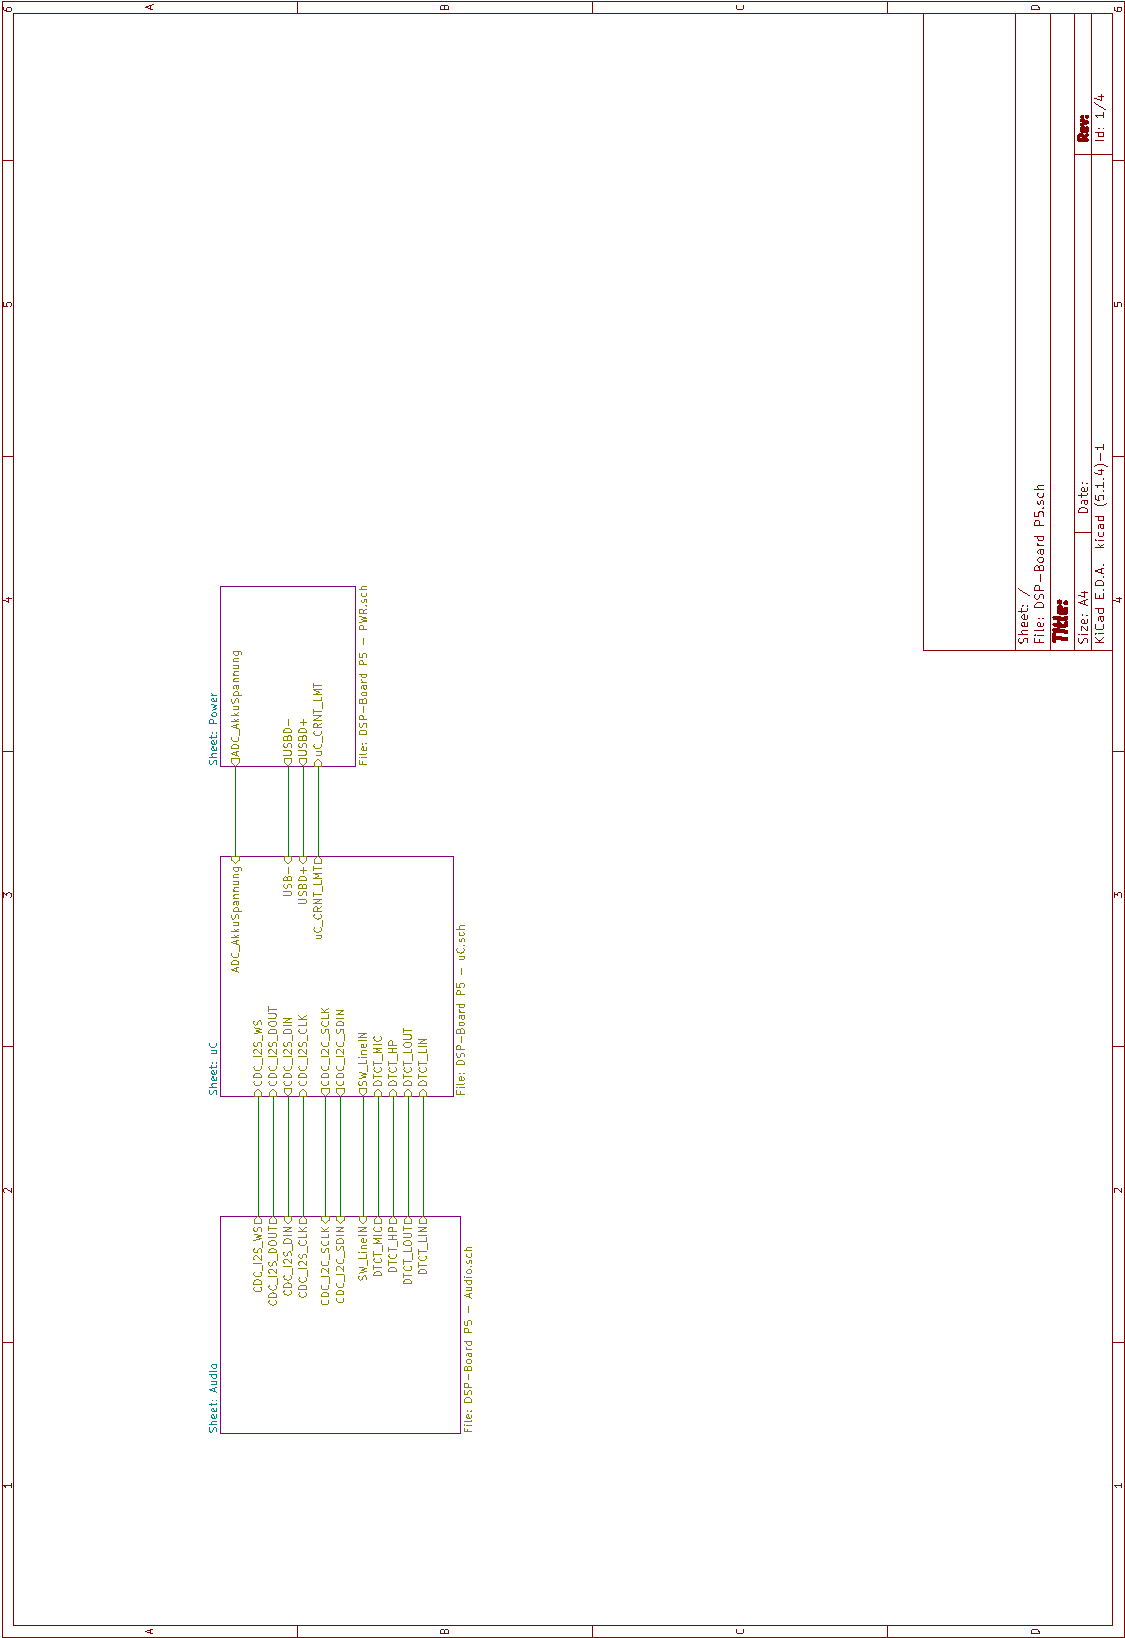
\includegraphics[width=0.95\linewidth]{appendix/DSP-Board-Schema-V1-1(1).pdf}
\end{figure}

\begin{figure}[h]
	\centering
	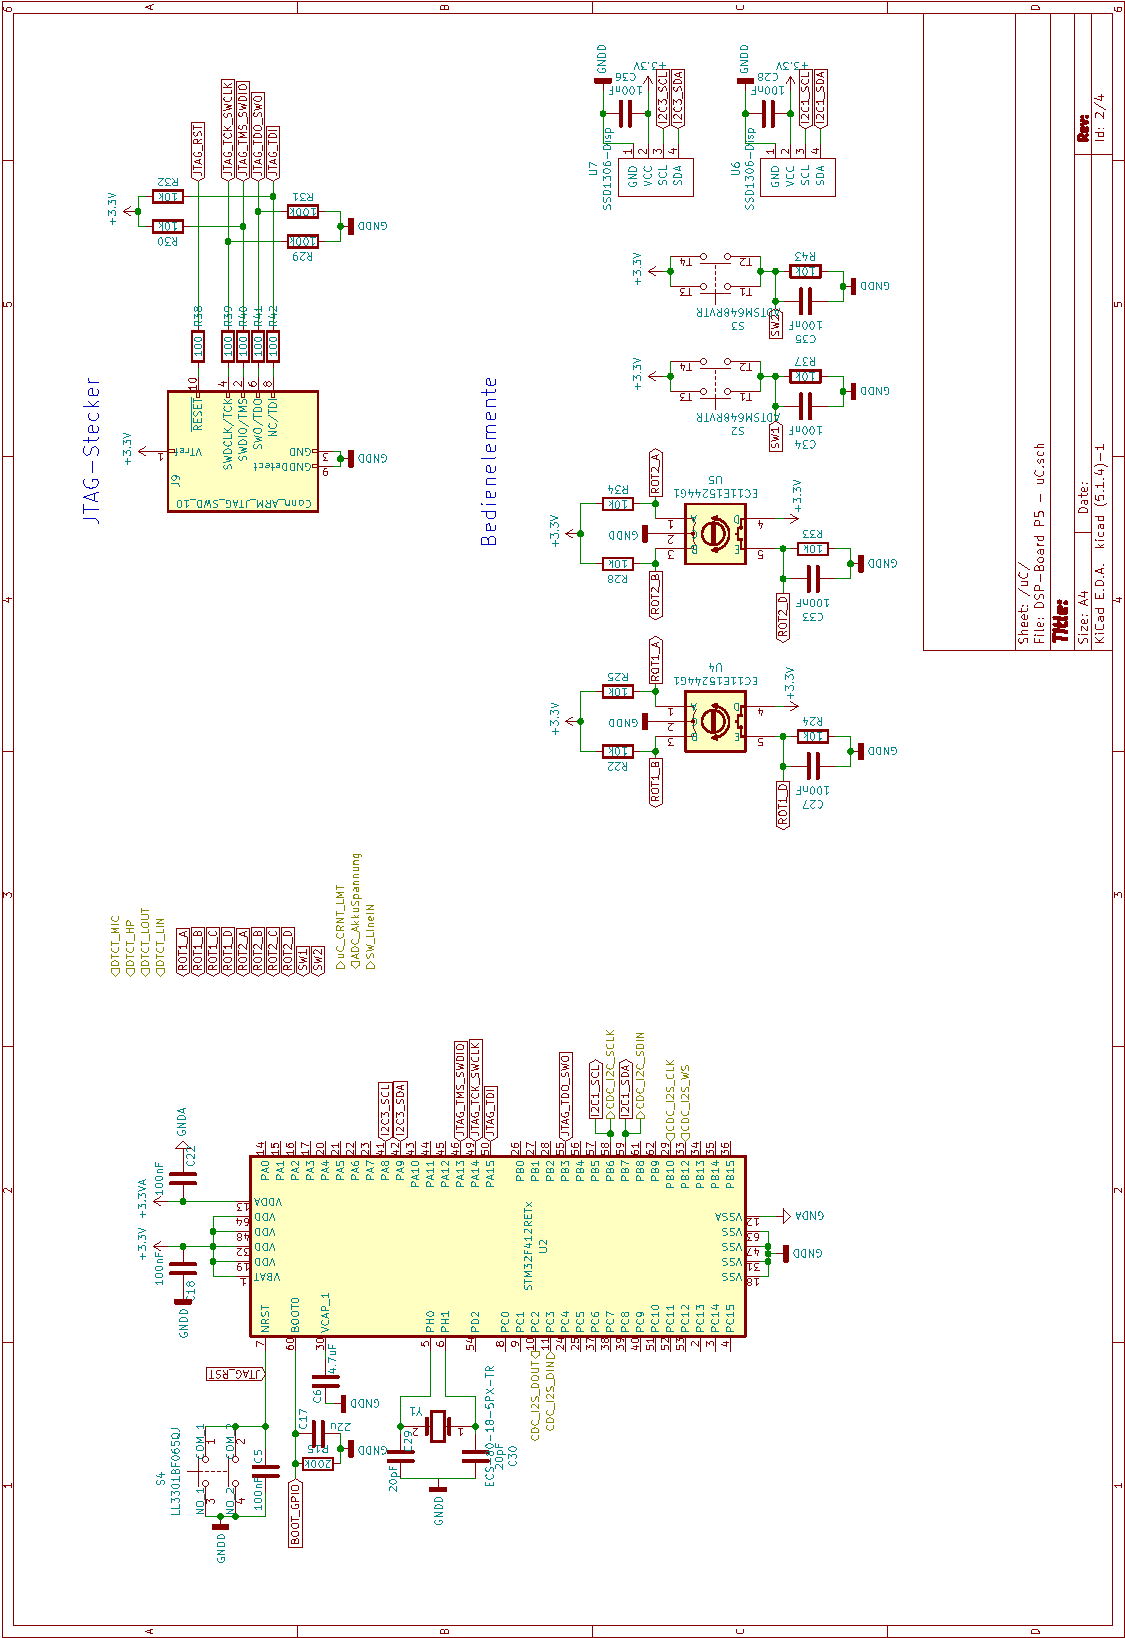
\includegraphics[width=0.95\linewidth]{appendix/DSP-Board-Schema-V1-1(2).pdf}
\end{figure}

\begin{figure}[h]
	\centering
	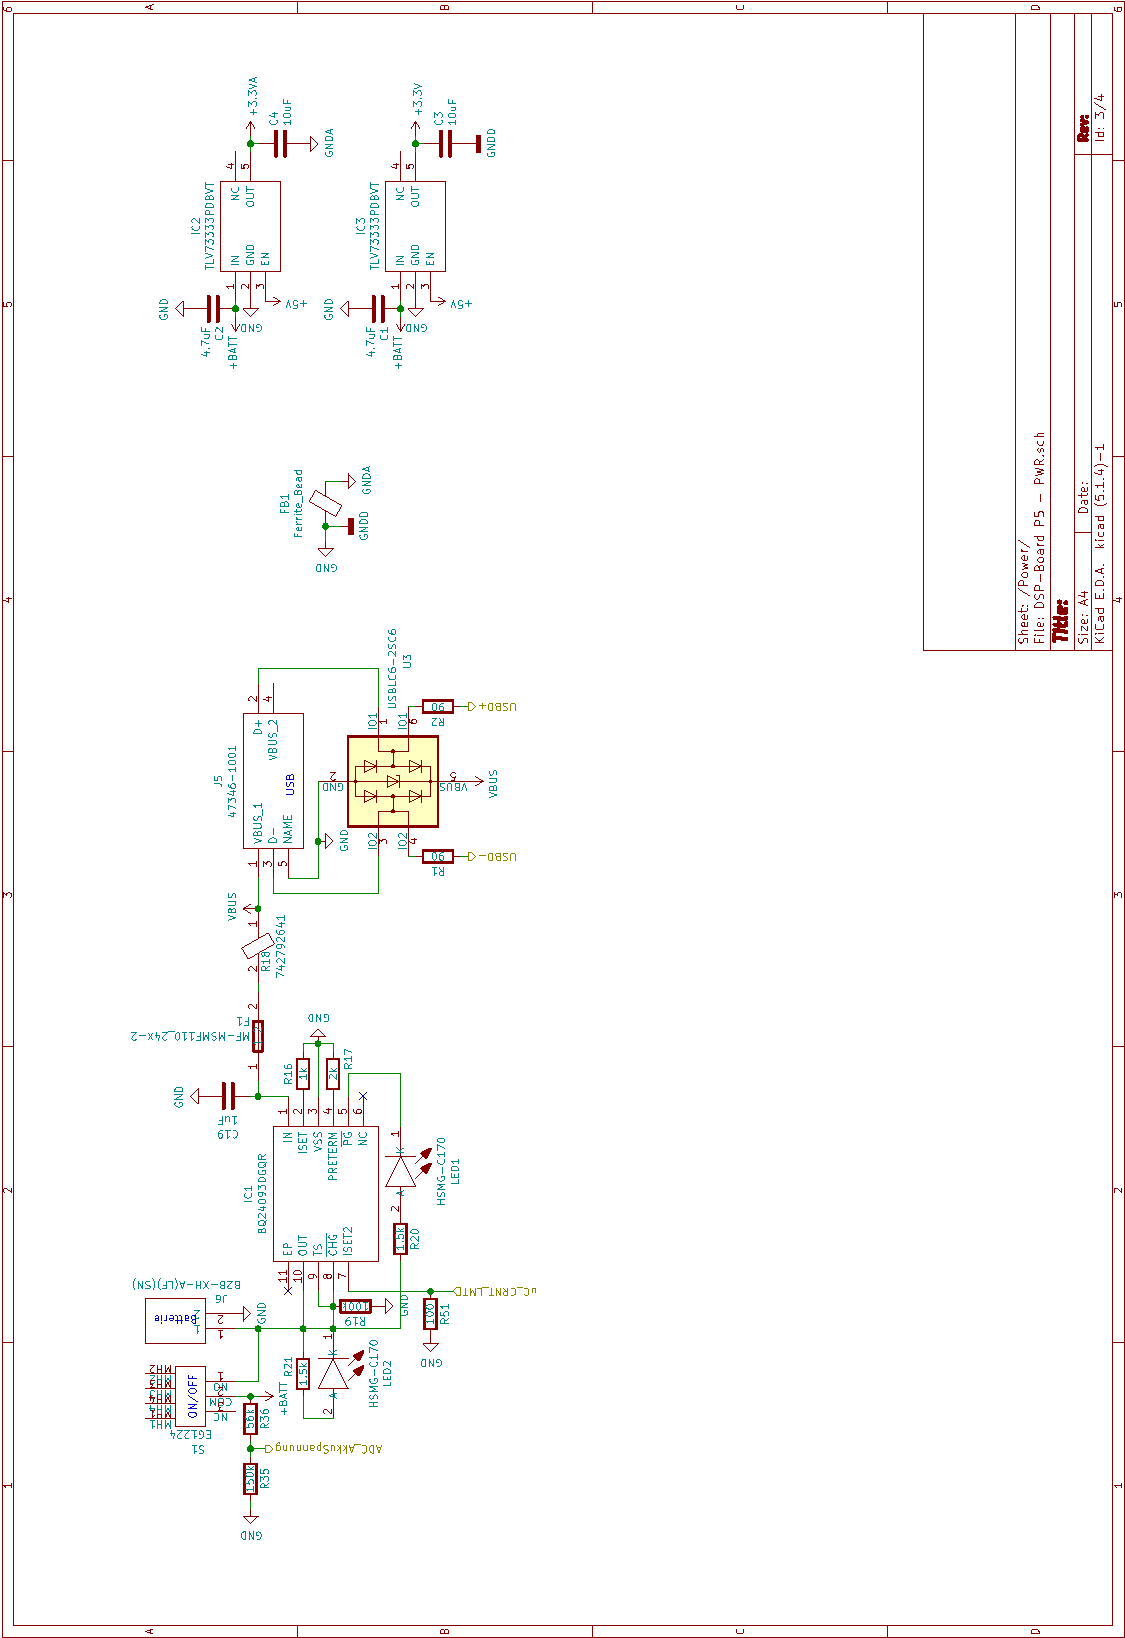
\includegraphics[width=0.95\linewidth]{appendix/DSP-Board-Schema-V1-1(3).pdf}
\end{figure}

\begin{figure}[h]
	\centering
	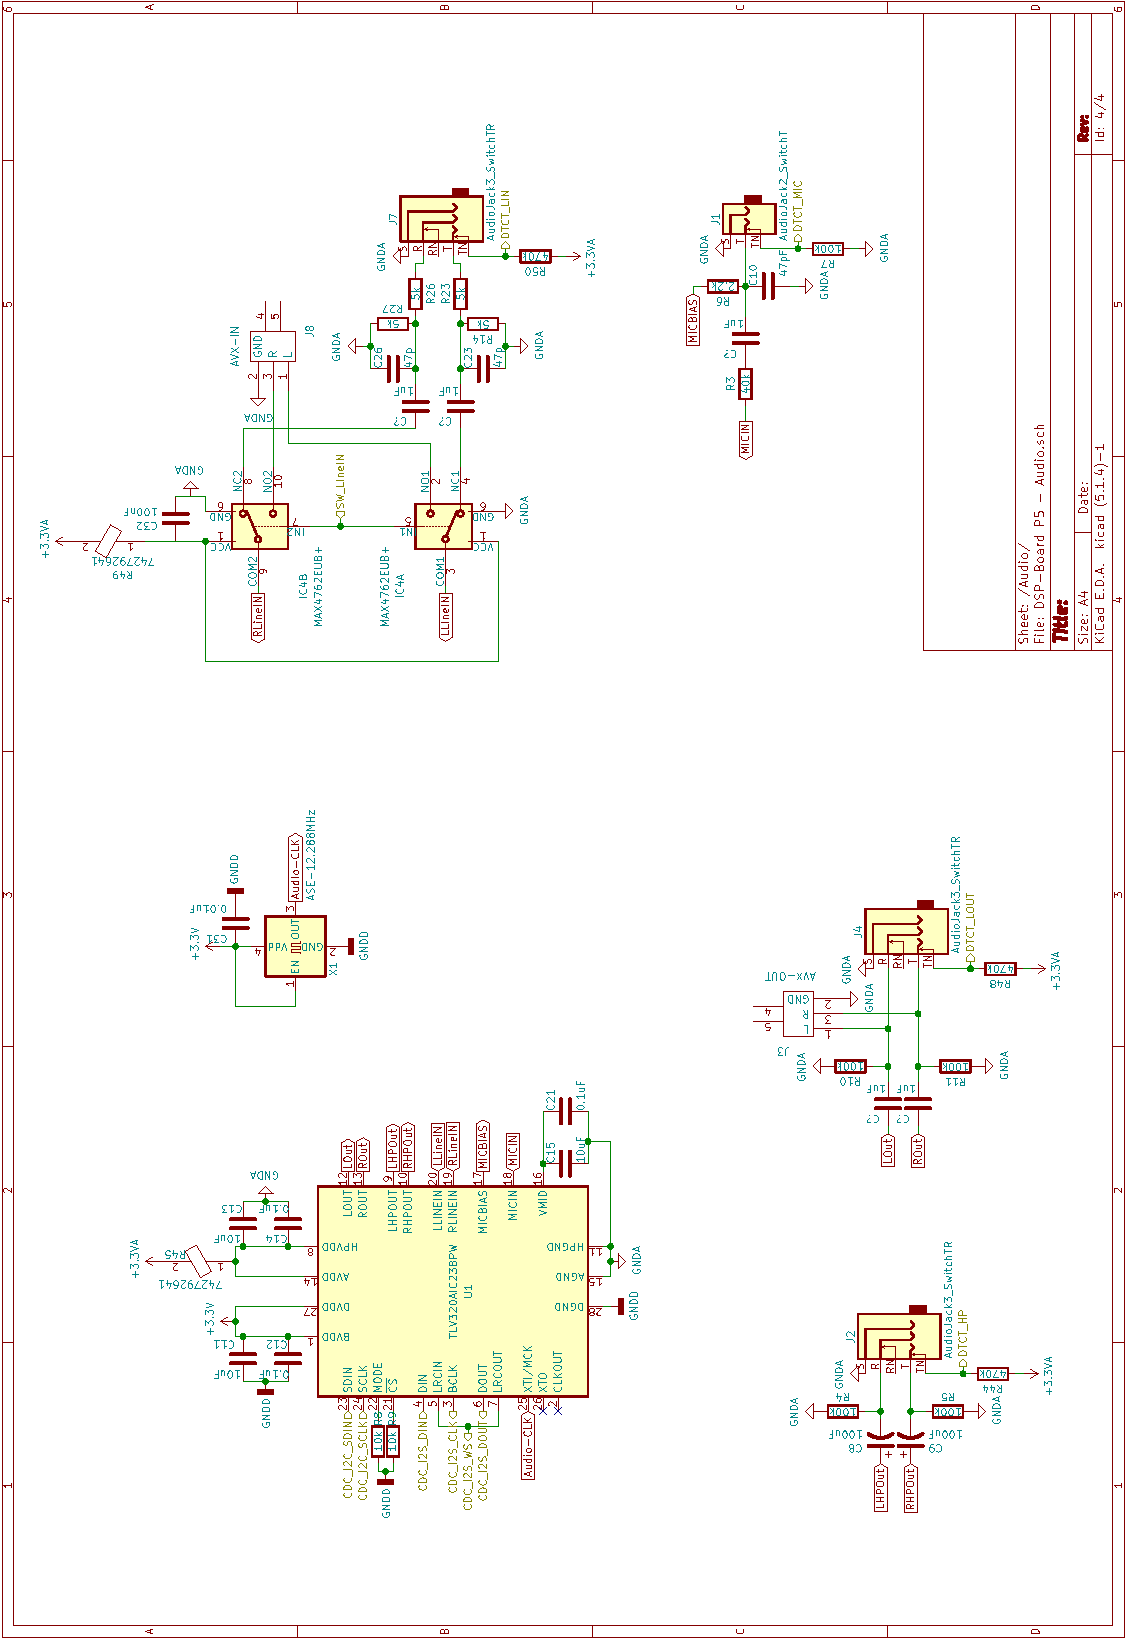
\includegraphics[width=0.95\linewidth]{appendix/DSP-Board-Schema-V1-1(4).pdf}
\end{figure}

\clearpage

\subsection{PCB Layout}
\label{app:PCB}

\begin{figure}[h!]
	\centering
	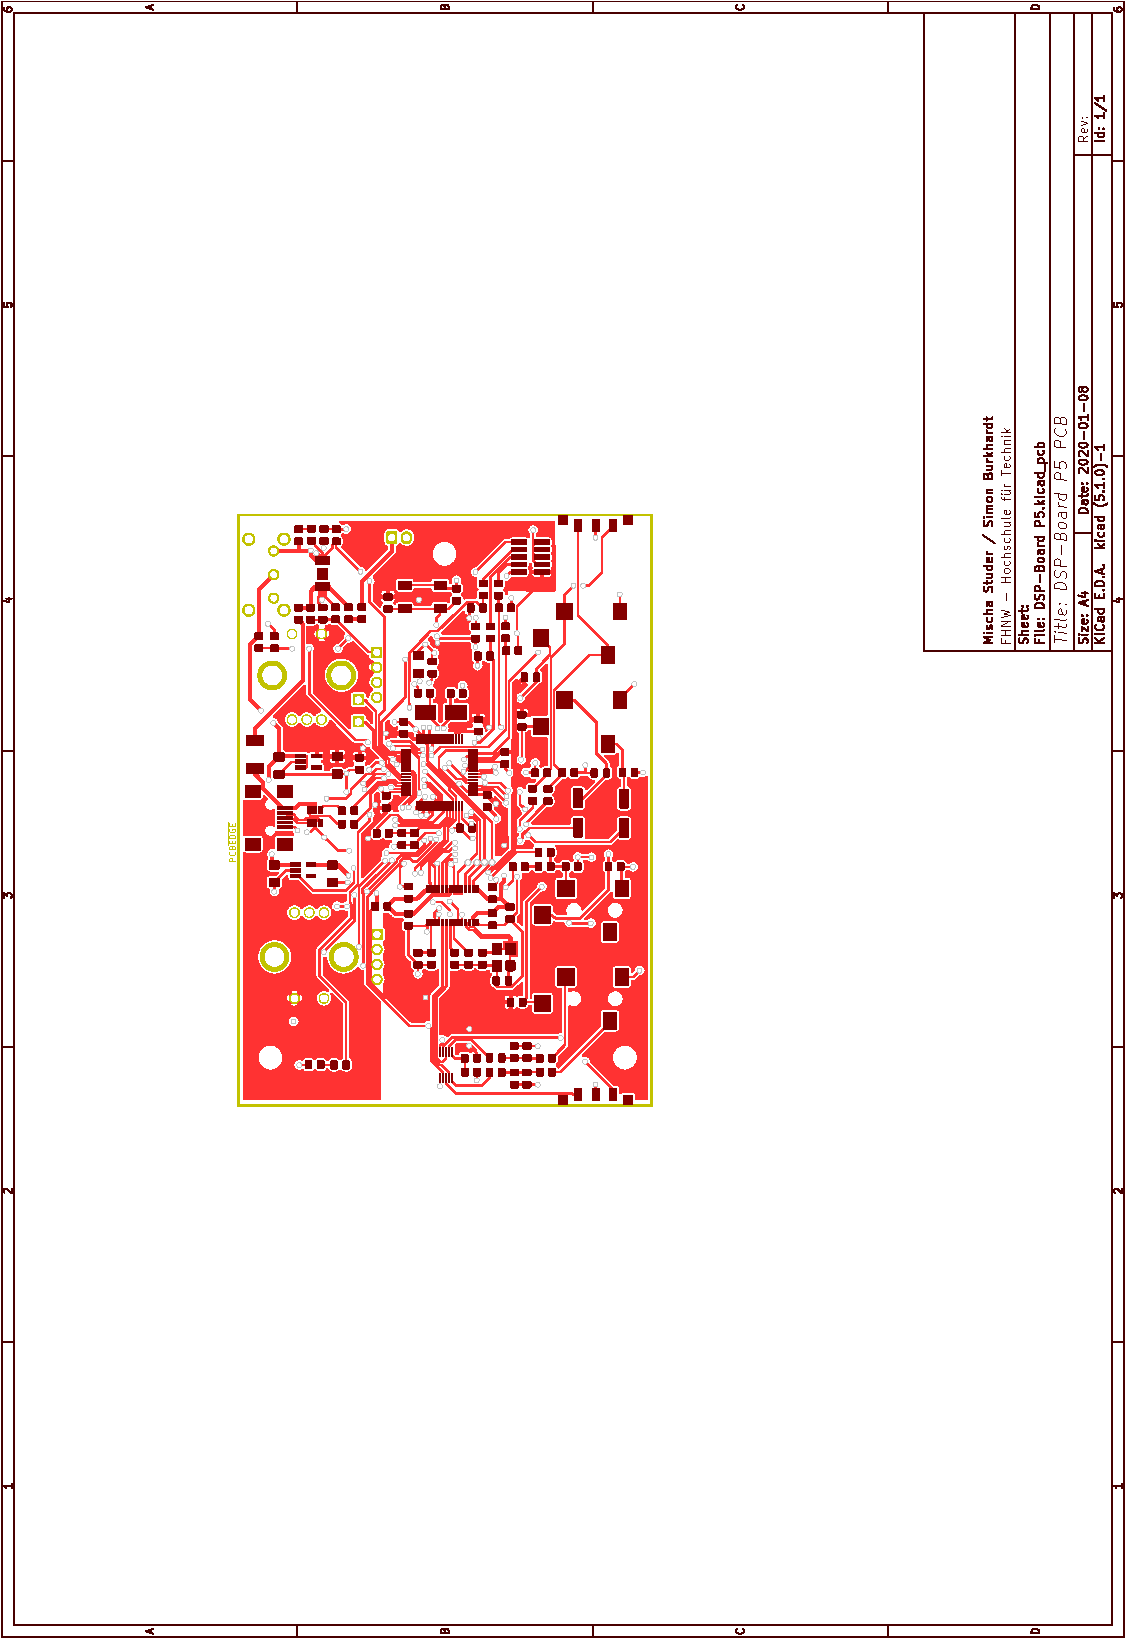
\includegraphics[width=0.95\linewidth]{appendix/DSP-Board-PCB-V1-1(1).pdf}
\end{figure}

\begin{figure}[h]
	\centering
	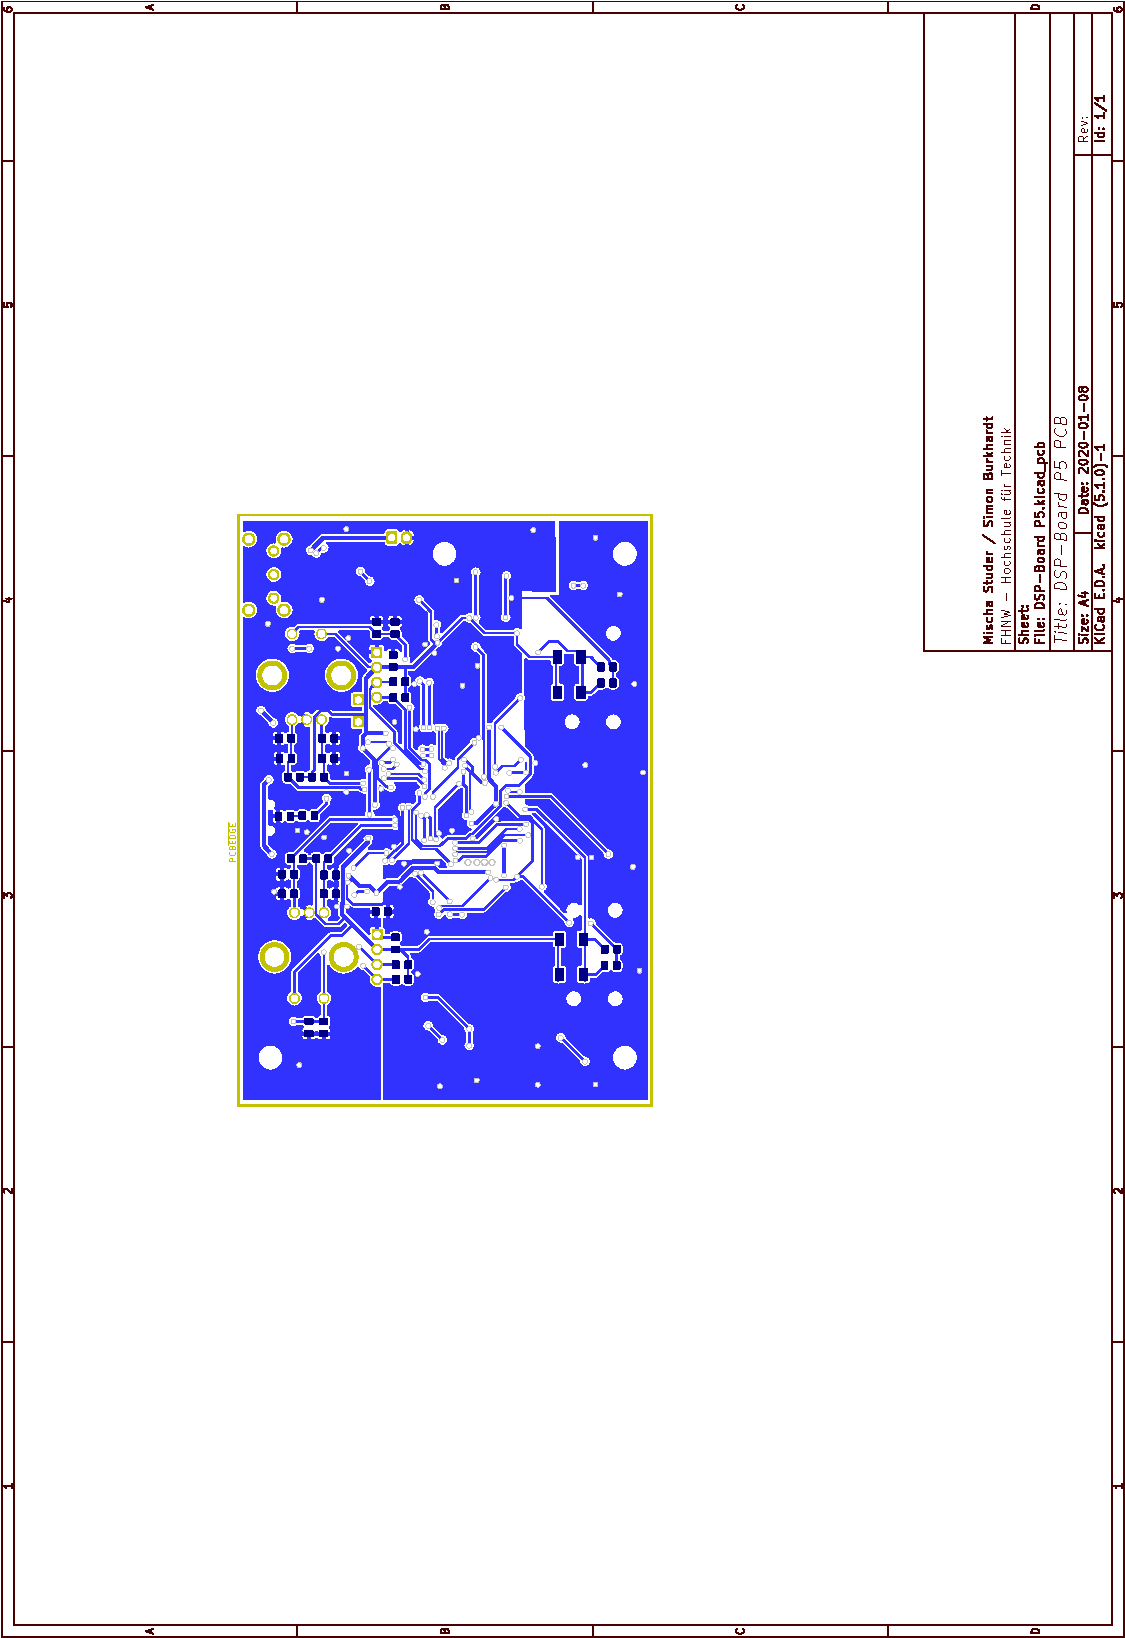
\includegraphics[width=0.95\linewidth]{appendix/DSP-Board-PCB-V1-1(2).pdf}
\end{figure}

\begin{figure}[h]
	\centering
	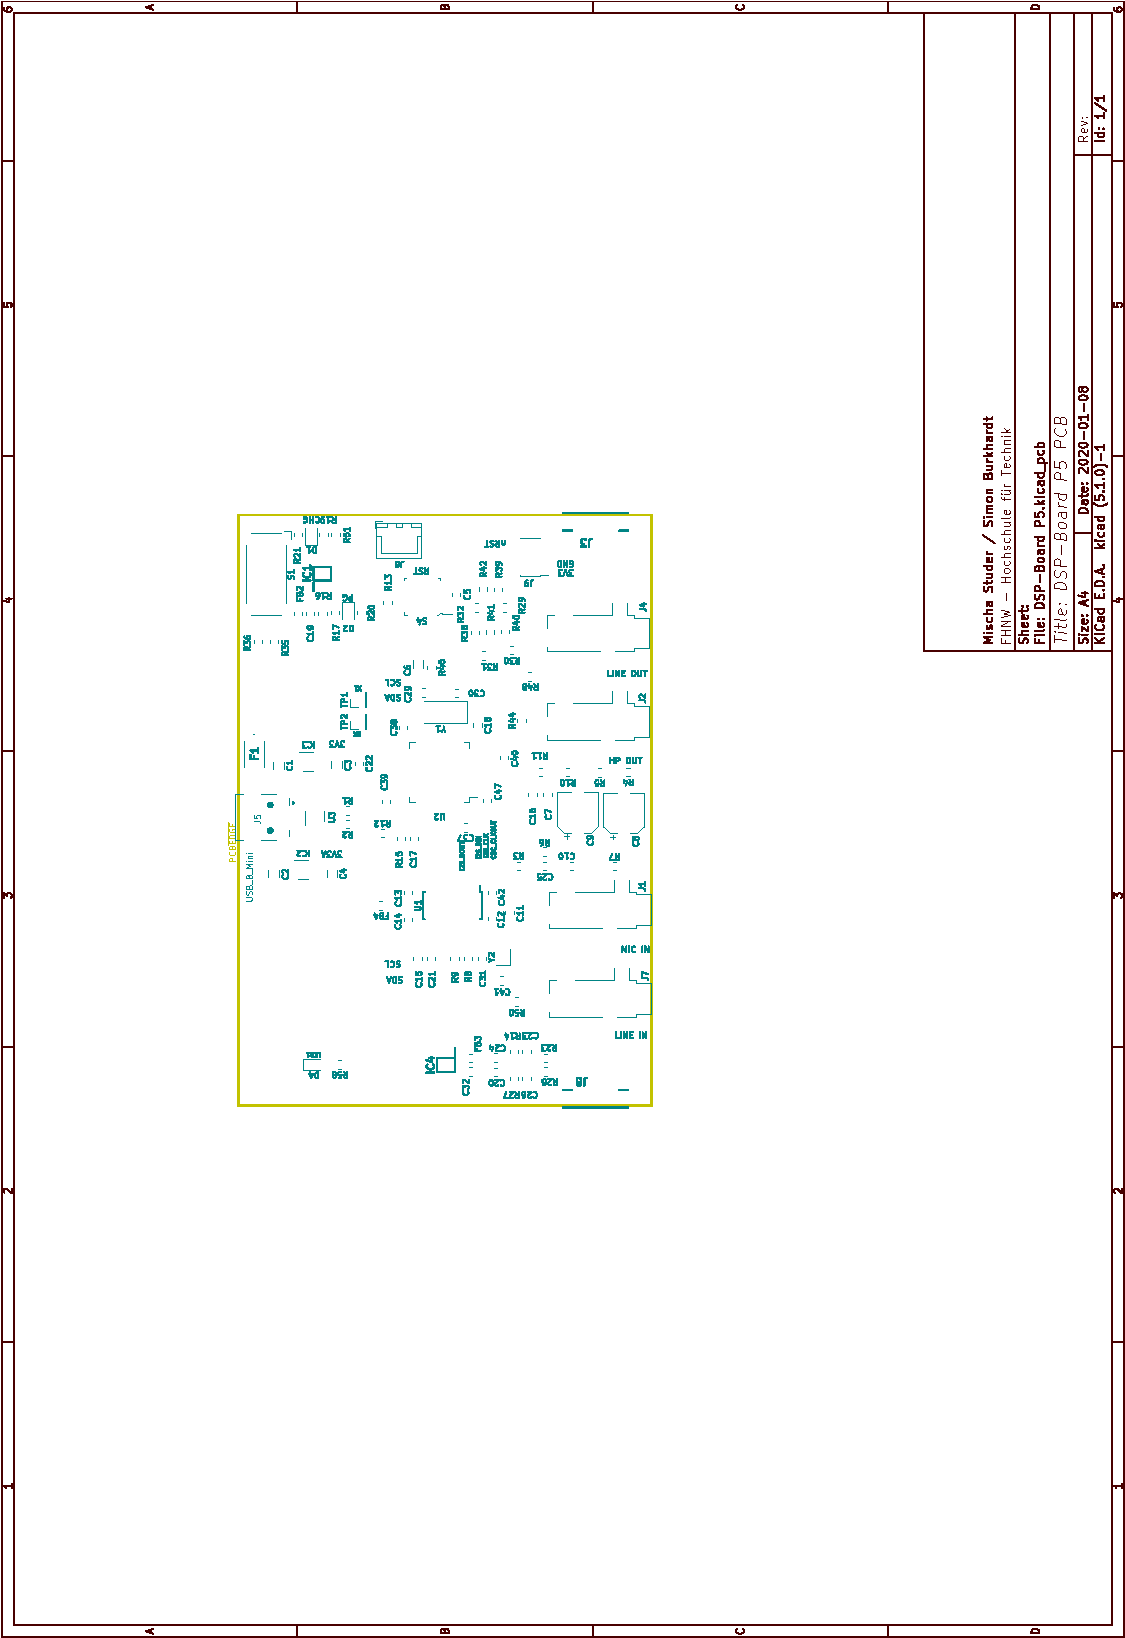
\includegraphics[width=0.95\linewidth]{appendix/DSP-Board-PCB-V1-1(3).pdf}
\end{figure}

\begin{figure}[h]
	\centering
	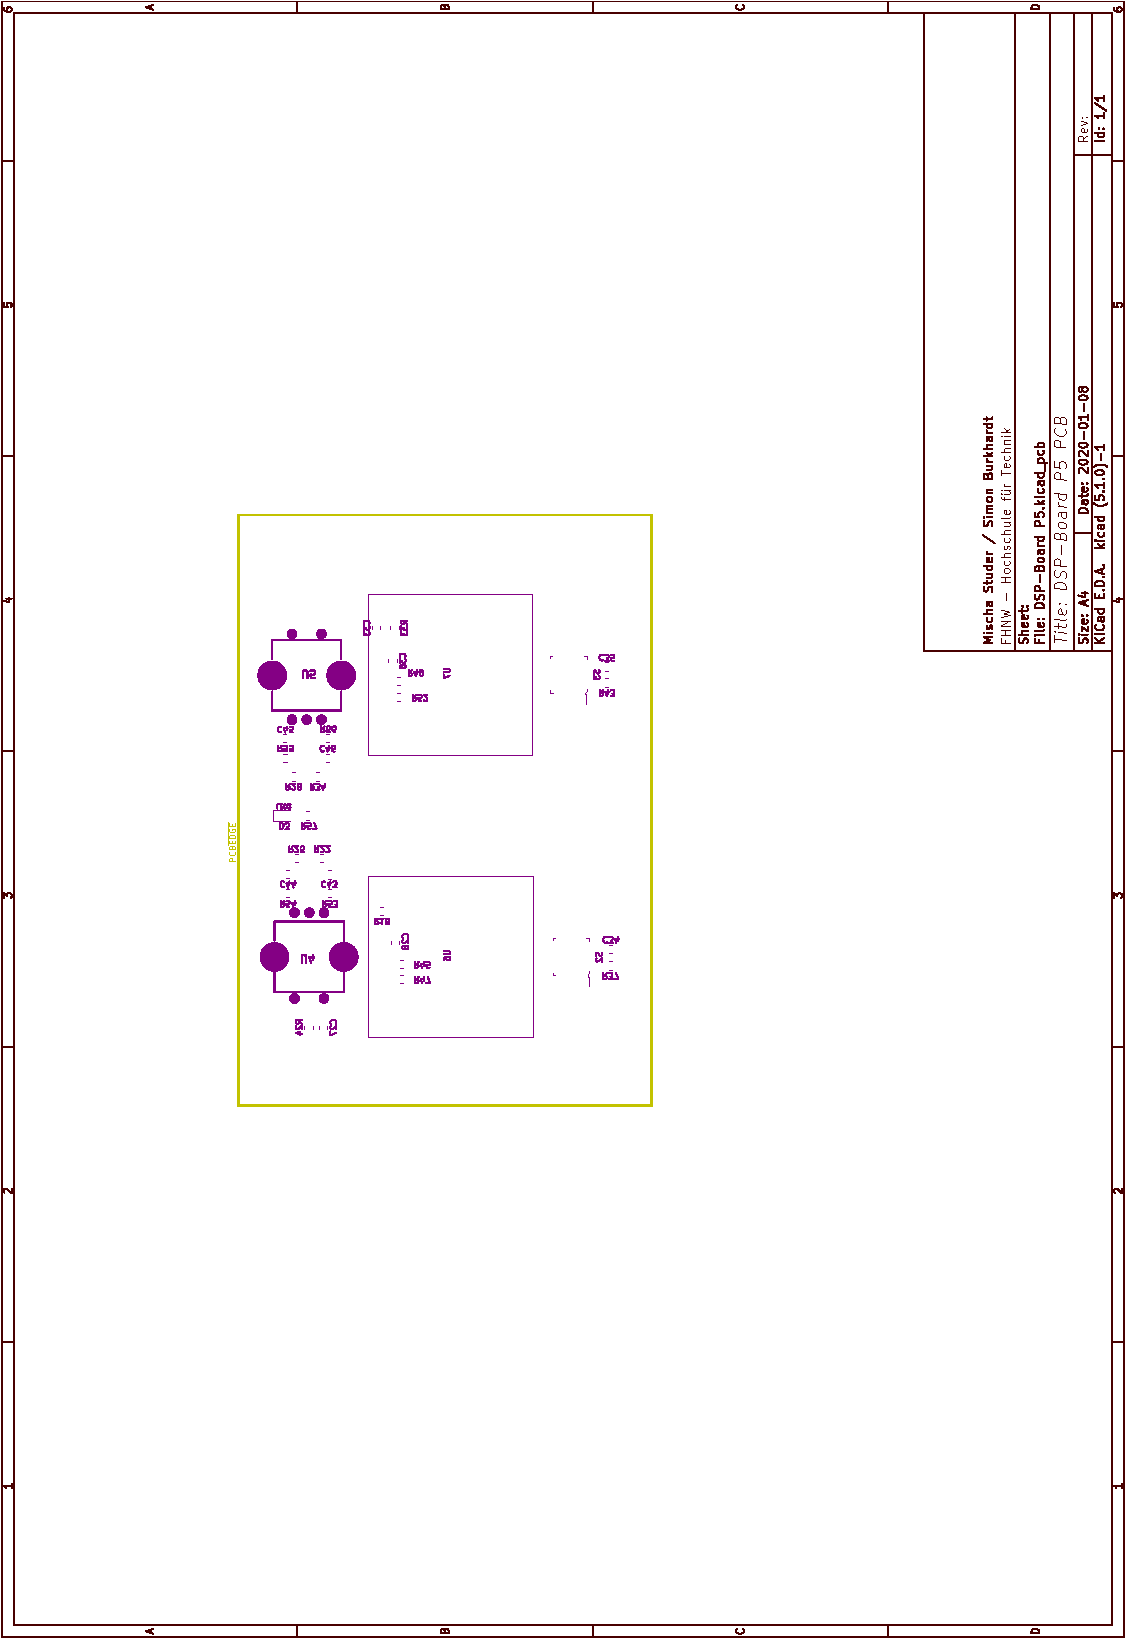
\includegraphics[width=0.95\linewidth]{appendix/DSP-Board-PCB-V1-1(4).pdf}
\end{figure}
\clearpage

\subsection{Pflichtenheft}
\label{app:Pflichtenheft}

\begin{figure}[h!]
	\centering
	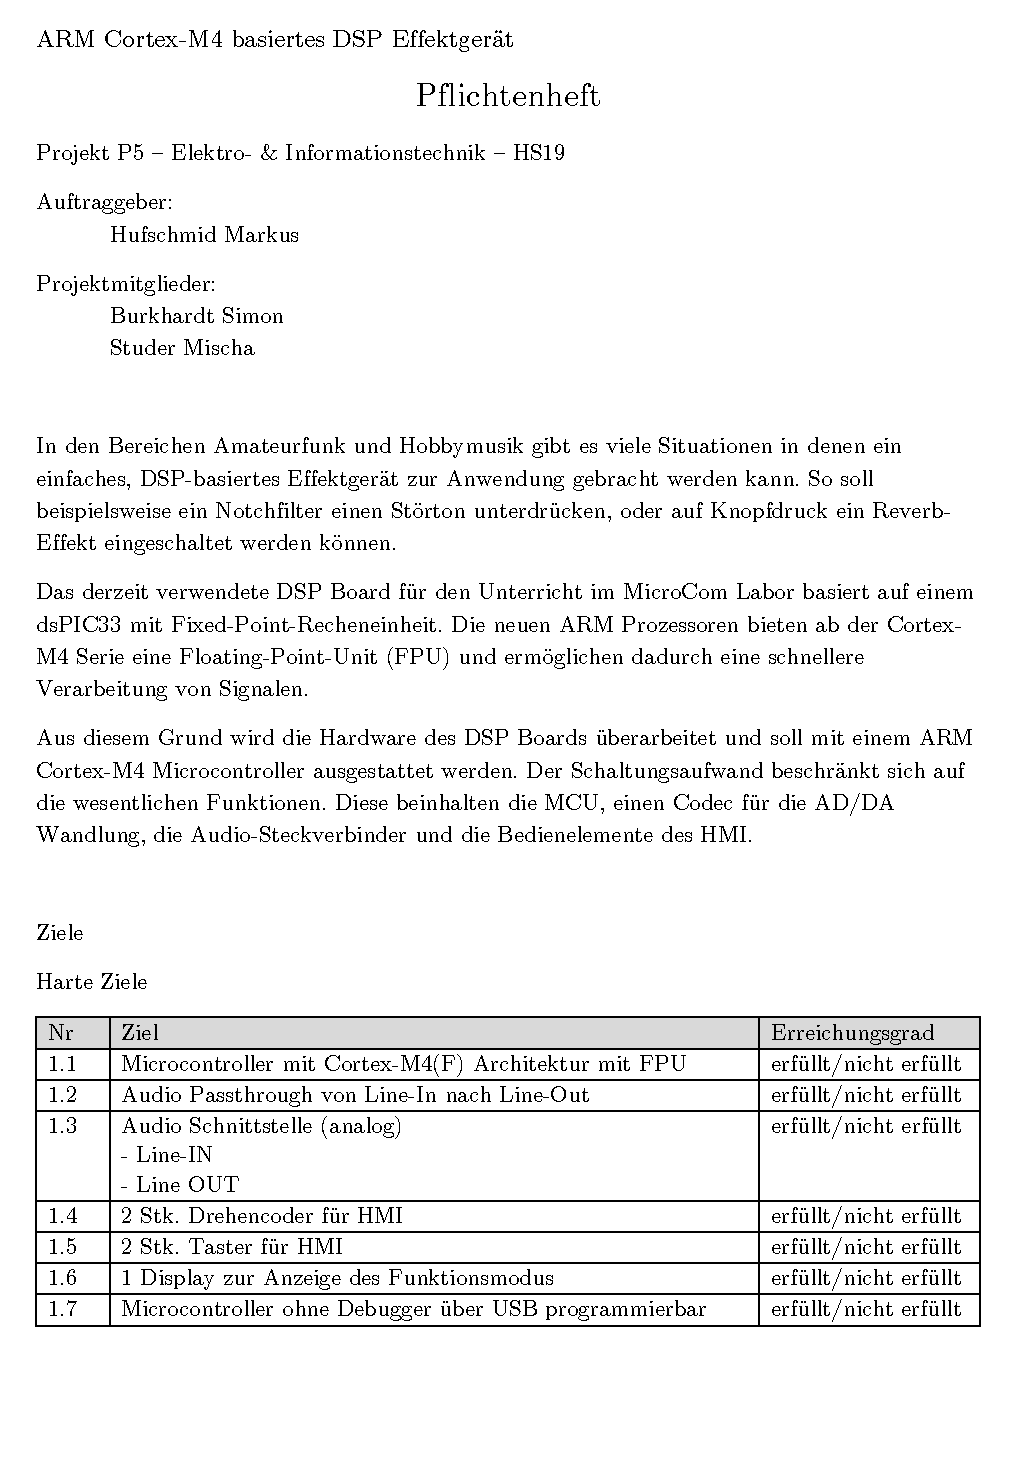
\includegraphics[width=0.95\linewidth]{appendix/pflichtenheft(1).pdf}
\end{figure}

\begin{figure}[h]
	\centering
	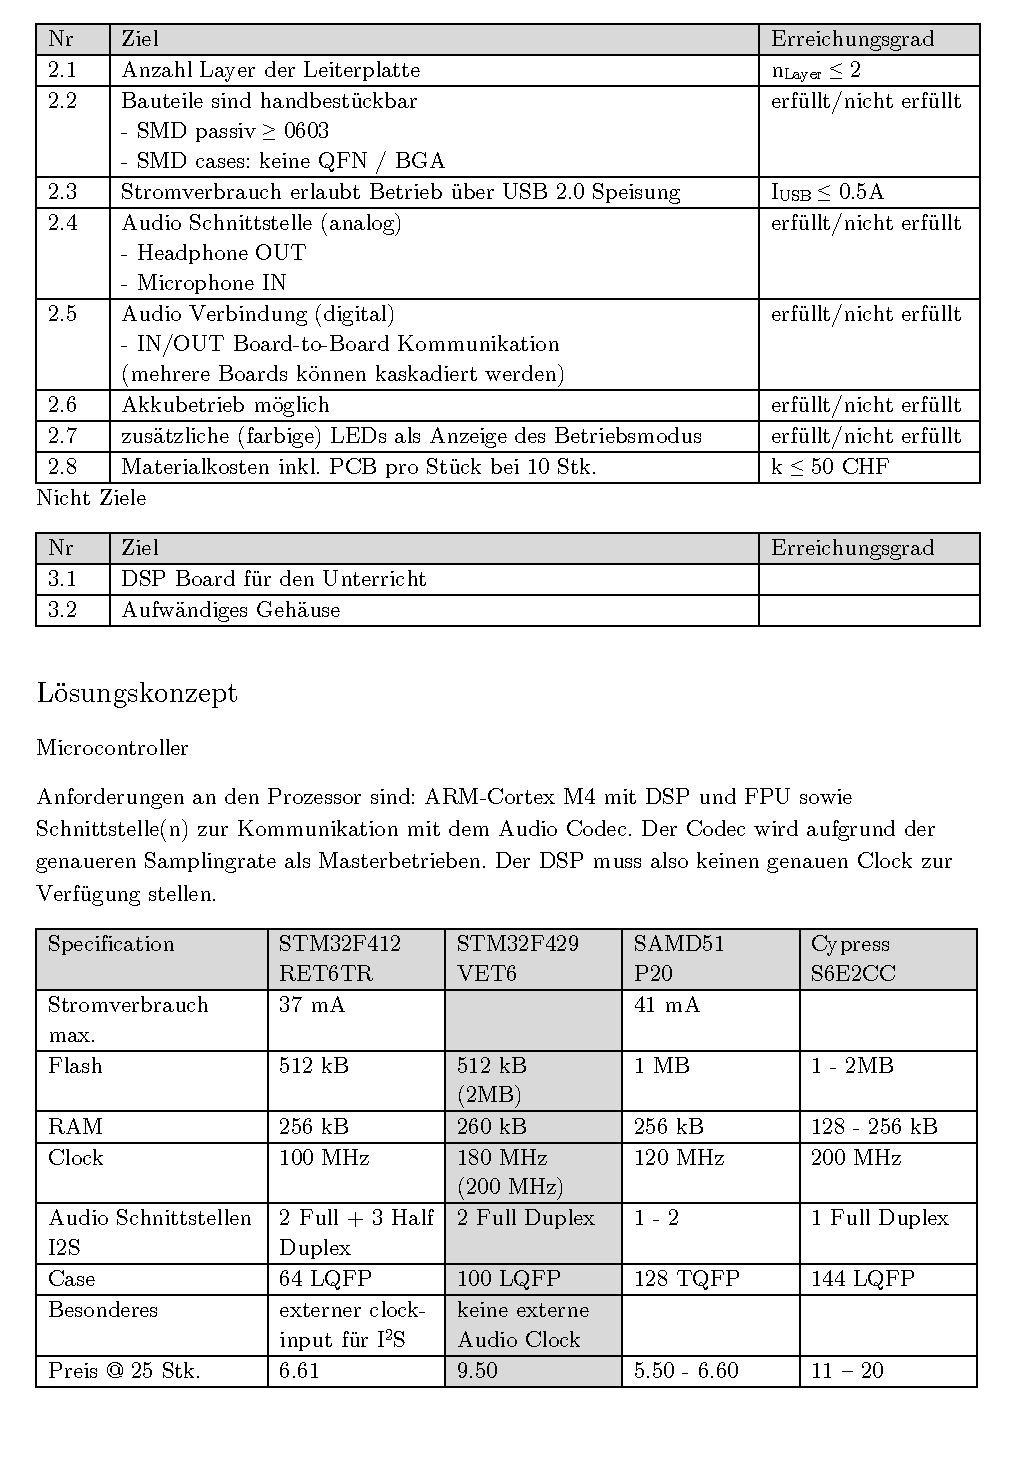
\includegraphics[width=0.95\linewidth]{appendix/pflichtenheft(2).pdf}
\end{figure}

\begin{figure}[h]
	\centering
	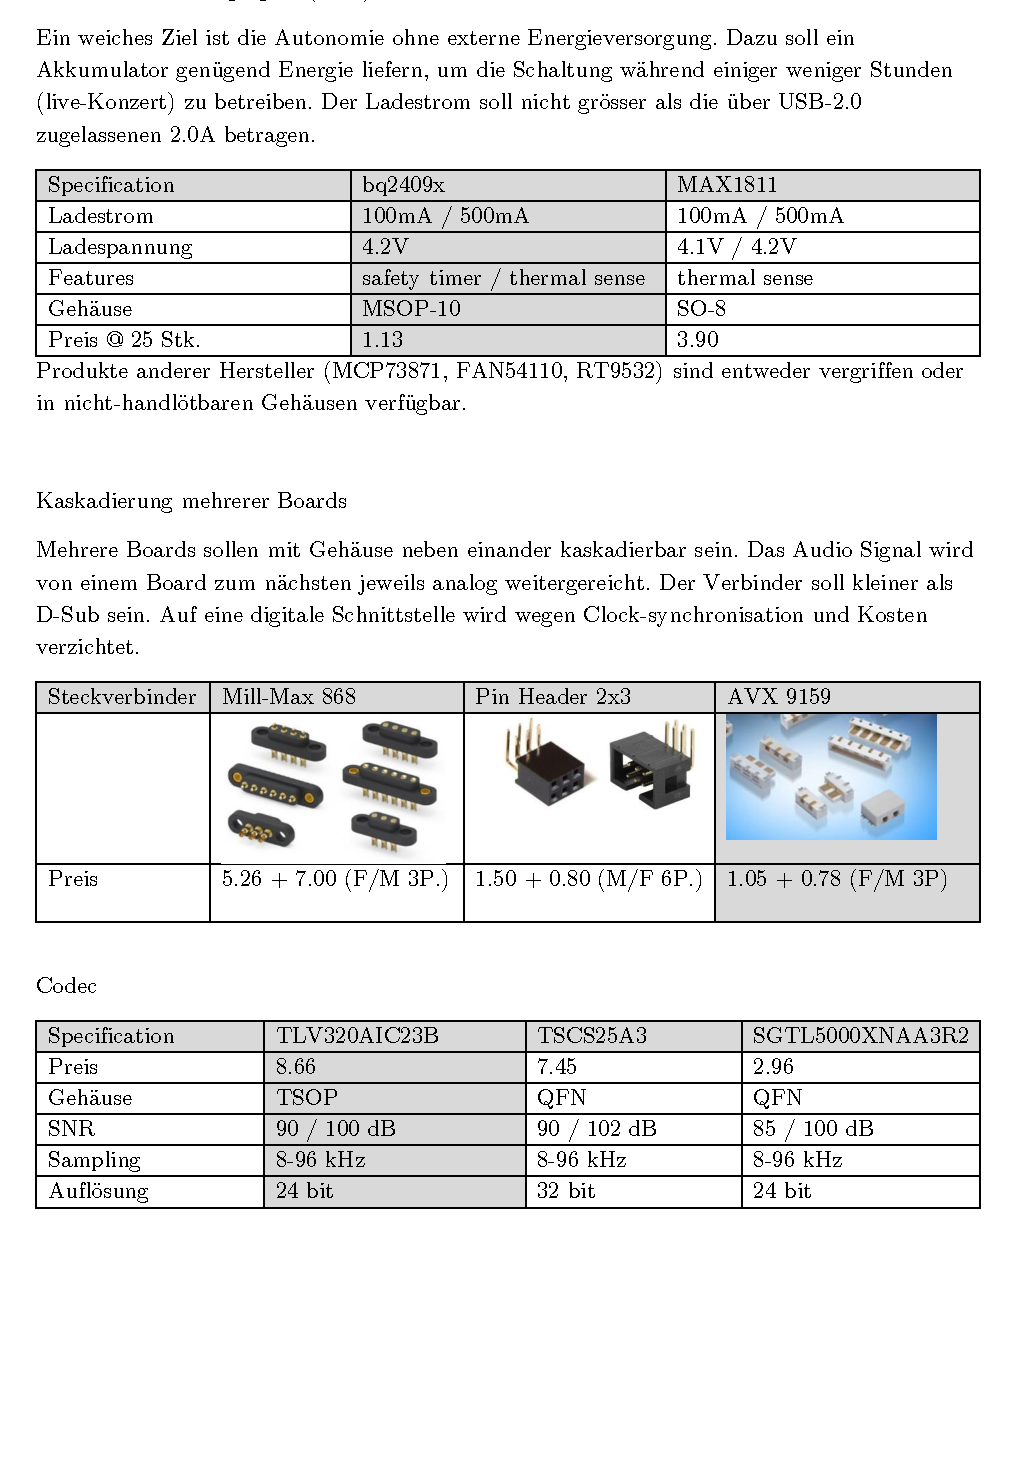
\includegraphics[width=0.95\linewidth]{appendix/pflichtenheft(3).pdf}
\end{figure}

\begin{figure}[h]
	\centering
	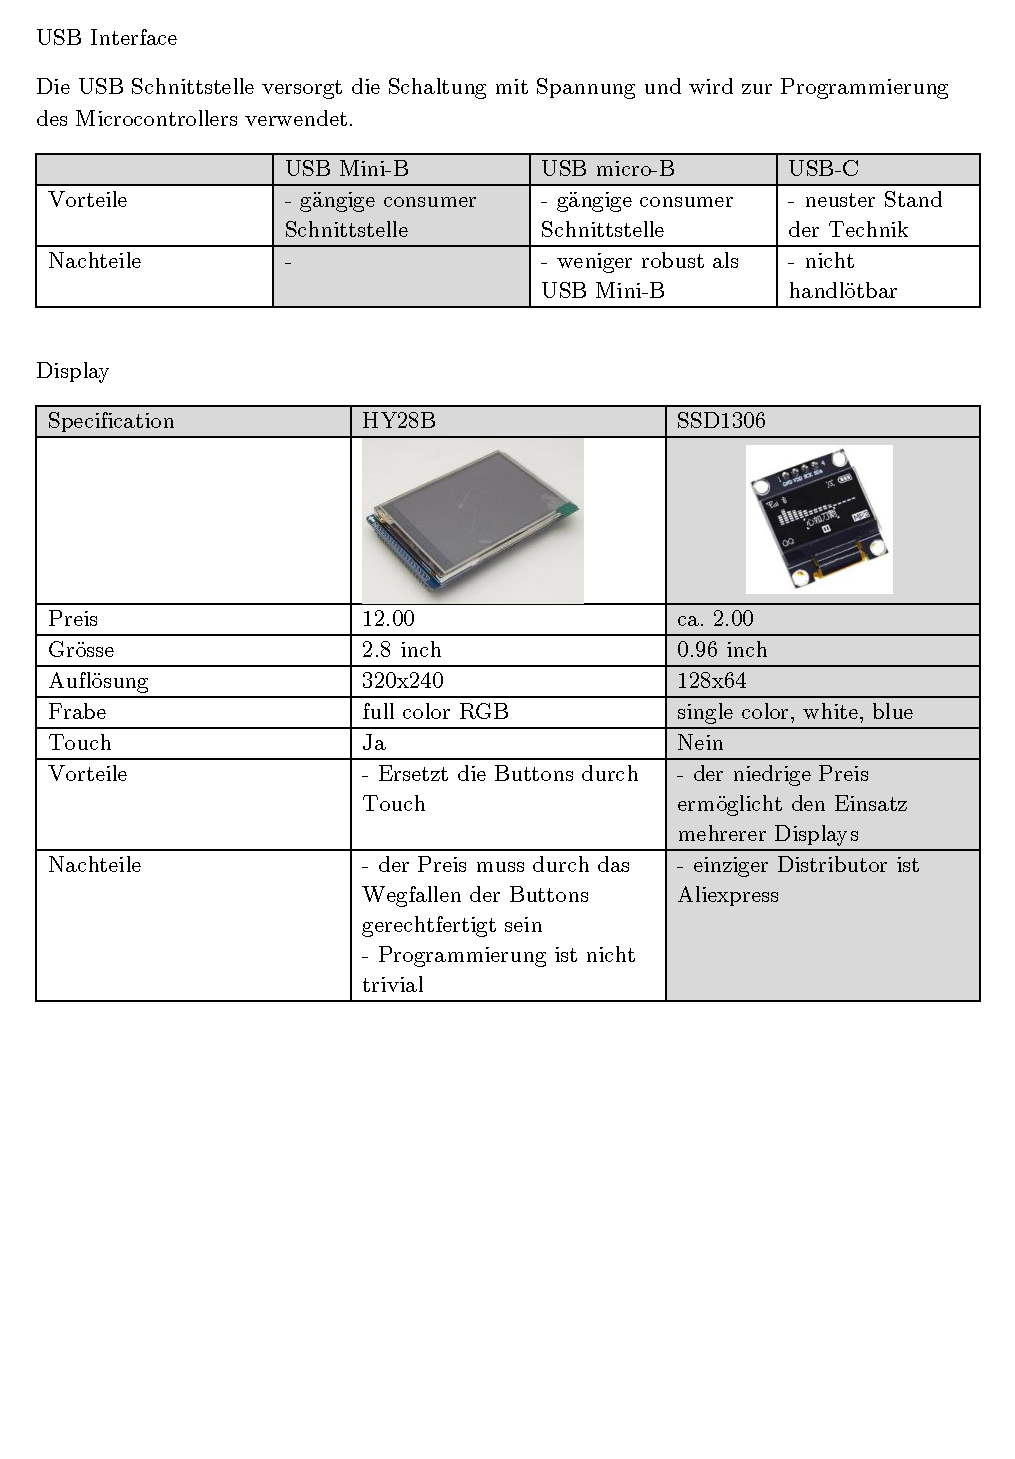
\includegraphics[width=0.95\linewidth]{appendix/pflichtenheft(4).pdf}
\end{figure}

\begin{figure}[h]
	\centering
	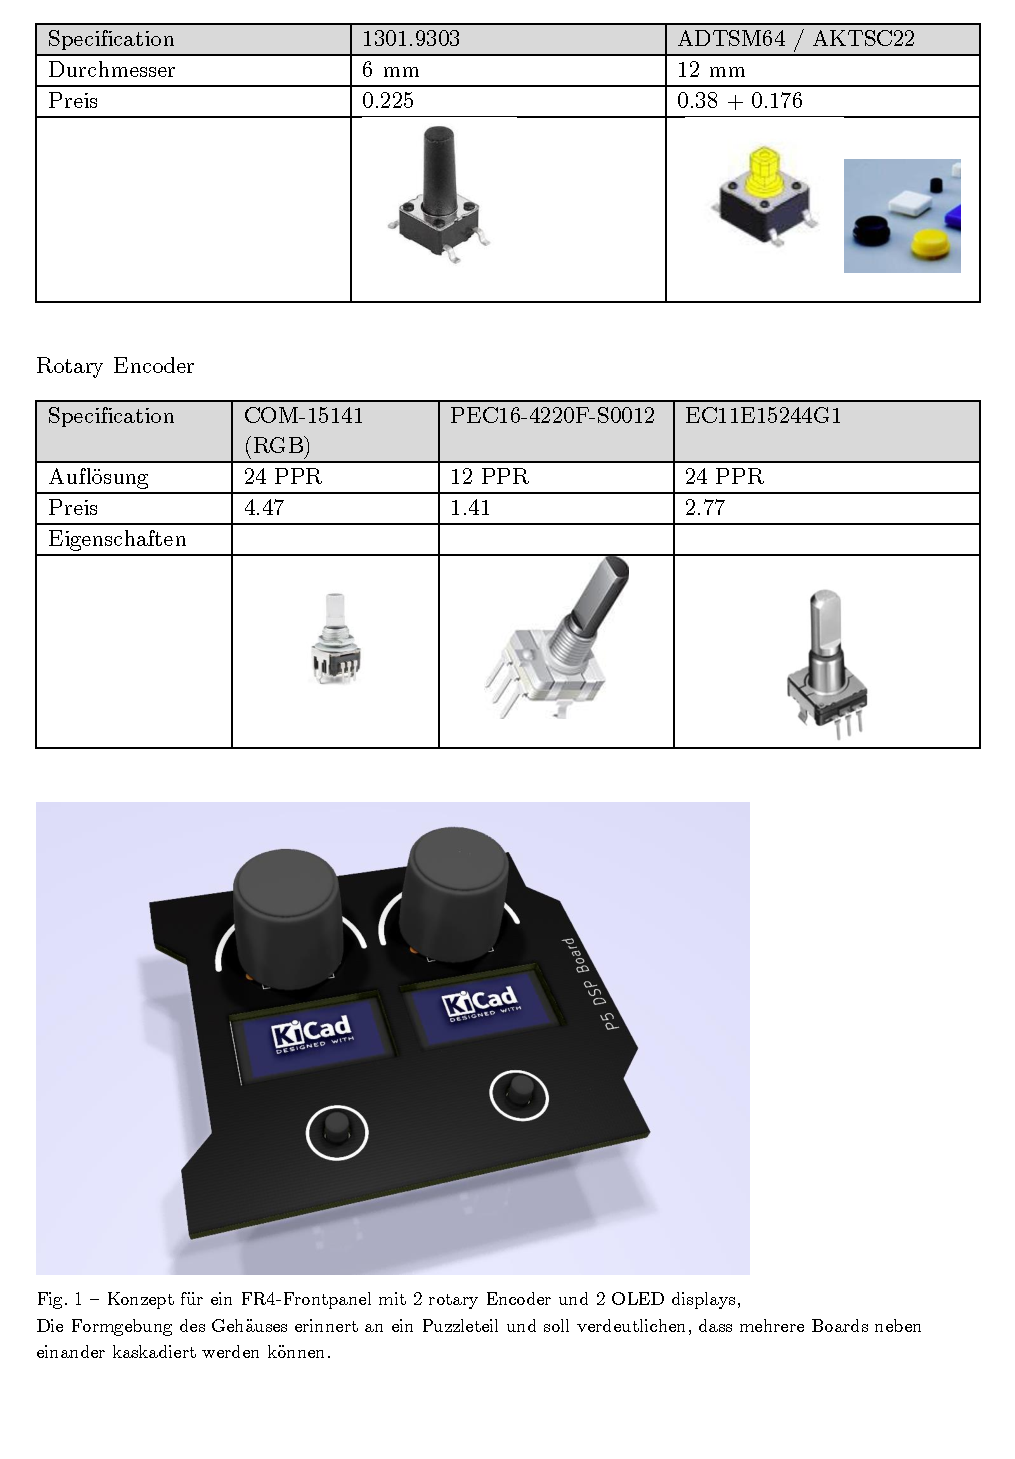
\includegraphics[width=0.95\linewidth]{appendix/pflichtenheft(5).pdf}
\end{figure}

\begin{figure}[h]
	\centering
	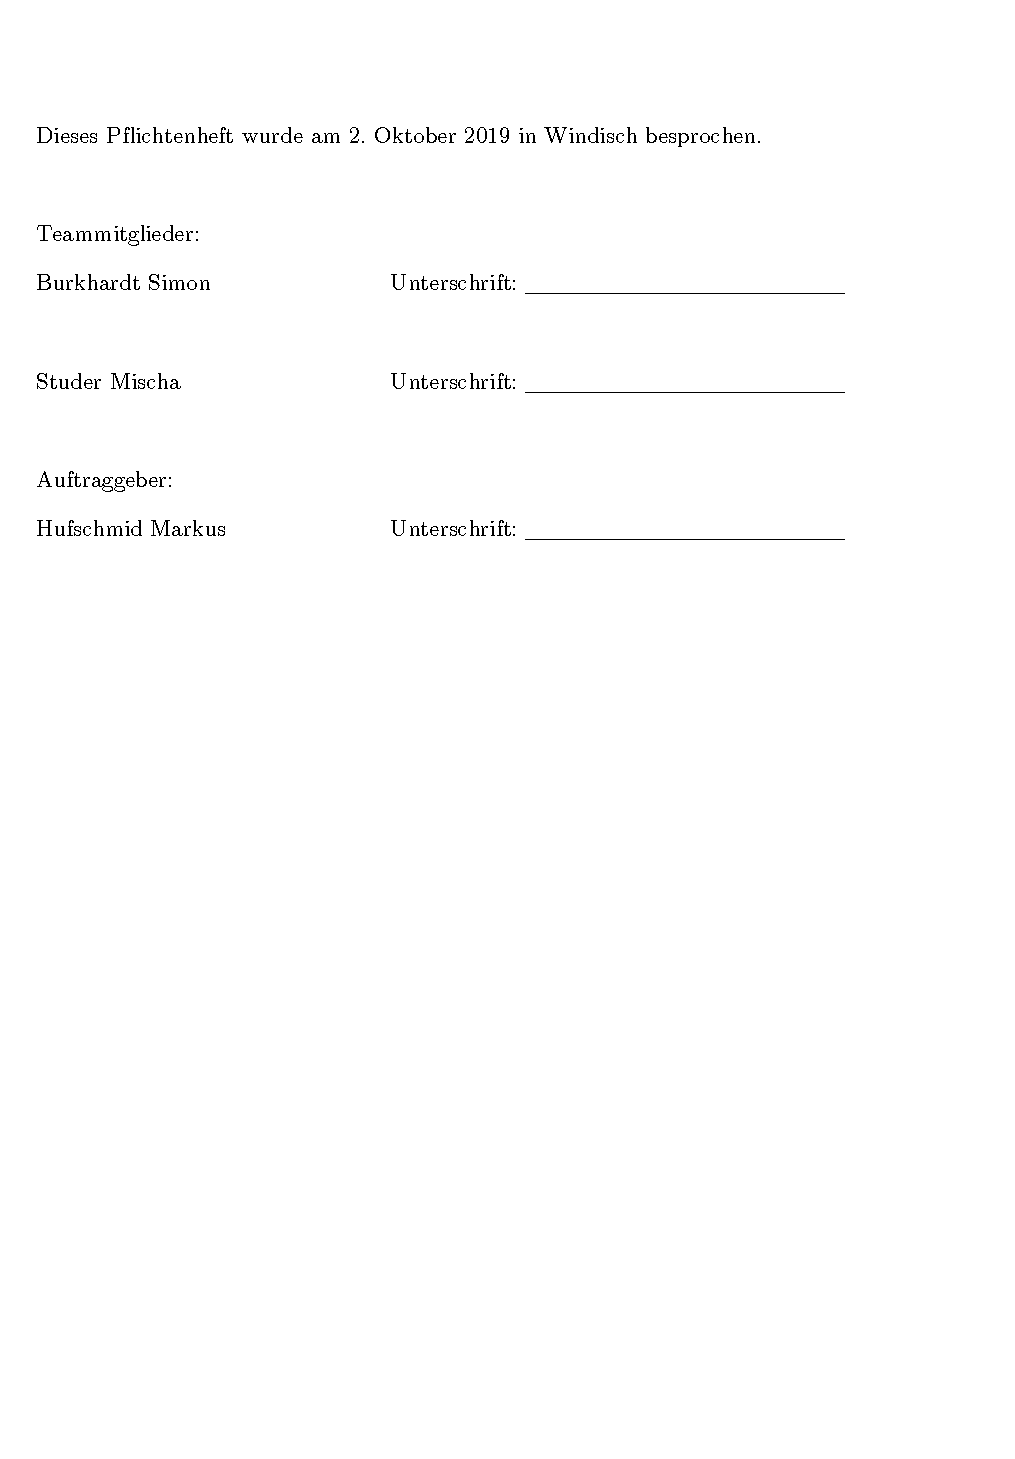
\includegraphics[width=0.95\linewidth]{appendix/pflichtenheft(6).pdf}
\end{figure}


\end{appendix}










%%---NOTES for DEBUG---------------------------------------------------------------------
%
\newpage
\listoftodos[\section{Todo-Notes}]
\clearpage


\end{document}